%%%%%%%%%%%%%%%%%%%%%%%%%%%%%%%%%%%%%%%%%%%%%%%%%%%%%%%%%%%%%%%%%%%%%%%%%%%%%%%
\section{Function approximation}\label{sec:mining}
%%%%%%%%%%%%%%%%%%%%%%%%%%%%%%%%%%%%%%%%%%%%%%%%%%%%%%%%%%%%%%%%%%%%%%%%%%%%%%%

The overall algorithm of function approximation is shown in figure~\ref{fig:approxAlg}
\begin{figure}[H]
\centering
\caption{Function approximation scheme}
\label{fig:approxAlg}
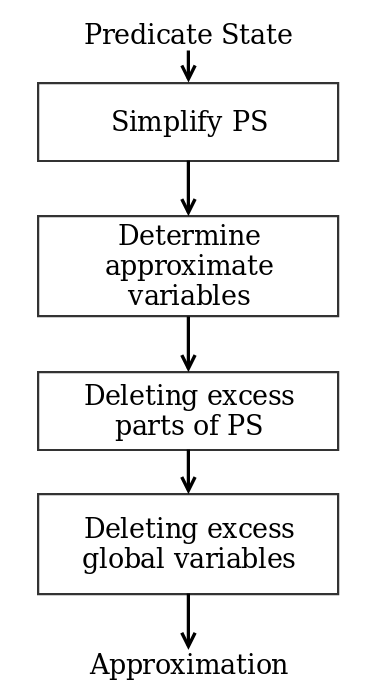
\includegraphics[keepaspectratio, width=\linewidth, height=8cm]{approxAlg}
\end{figure}


\subsection{Predicate State simplify}
At the beginning we must simplify predicate state, because LLVM uses static single assignment form (SSA), what complicates approximation. There are 2 simplify rules:
\begin{itemize}
\item if right side of current predicate equal or contained in left side of previous predicate, then we replace right side of current predicate by right side of previous;
\item for path predicates always replace value in condition by what was previously assigned
\end{itemize} 
An example of PS simplifying is shown in figure~\ref{fig:simEx}

\begin{figure}[tbh]
\centering
\caption{Function simplify example}
\label{fig:simEx}
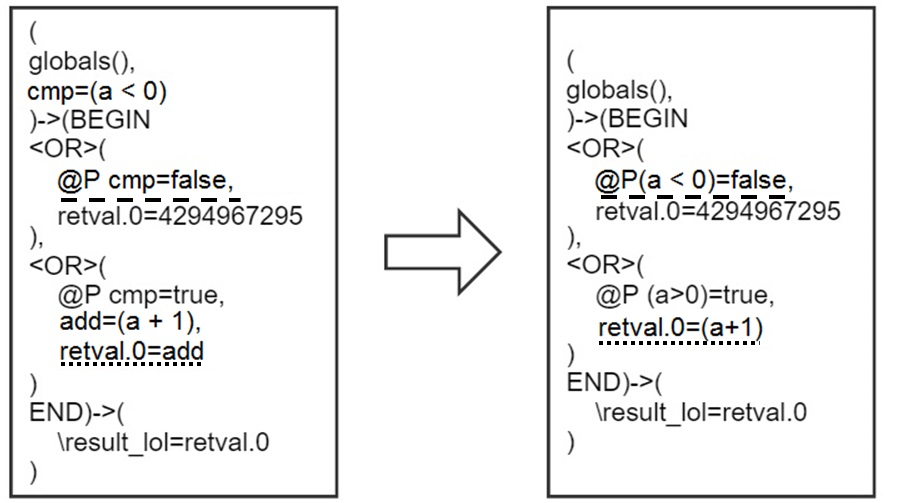
\includegraphics[keepaspectratio, width=8cm, height=7cm]{ex2}
\end{figure}

\subsection{Determine approximate variables}
After simplifying we must to decide over which variables we will be approximate. In this work we decide to approximate over variables, which lead return values to constants. These variables are in path predicates on one of the branches which assigned the return value to the constant. This is done using algorithm~\ref{alg:approx}.

\begin{algorithm}[tbh]
\caption{Determining of approximating variables}
\label{alg:approx}

\textbf{Input:}  $P_i$  --- current predicate\\
\textbf{Input:}  $rtv$  --- return value\\
\textbf{Output:} $PrPred$ --- approximated predicates

\begin{algorithmic}
\If {$getType(P_i) = Path$}
    \State $curPath \Leftarrow P_i$
\EndIf
\If {$getLhv(P_i)~=~rtv$~\&\&~!$isOpaqueTerm(getRhv(P_i))$}
    \State $PrPred \Leftarrow PrPred \cup curPath$ 
\EndIf
\end{algorithmic}
\end{algorithm}

\subsection{Deleting excess parts of PS}
After determining approximate variables we need to extract parts of predicate state, which have influence on approximate variables. For this, first we must to traverse direct acyclic graph~(DAG) of program until we meet path predicate, which chose on previous step. Next we perfome reverse traverse with saving all code pieces.

For that algorithm we developed a mechanism of DAG traverse, which can consider all predicate state and it's distinct parts in direct and reverse order. After extracting we must to simplify predicate state by deleting unused global variables and empty constructions. This is done using algorithm~\ref{alg:deleting}

\begin{algorithm}[tbh]
\caption{Deleting unused global variables}
\label{alg:deleting}

\textbf{Input:}  $P_i$  --- current predicate\\
\textbf{Output:} $ProtTerms$ --- protected terms

\begin{algorithmic}
\State $lhv \Leftarrow getLhv(P_i)$
\If {$lhv \in Global$}
    \State $lhvTerms \Leftarrow getFullTermSet(lhv)$
    \If {$protTerms \cap lhvTerms$}
    	\For{$rhv \in getRhv(P_i)$}
    		\State $protTerms \Leftarrow protTerms \cup rhv$ 
    	\EndFor
    \EndIf
\EndIf
\end{algorithmic}
\end{algorithm}

The result of function approximation is stored in new type of predicate state named predicate state imply, which have the next logic interpretation: $A \implies B$. Example of how function approximation can prove static analysis is shown in figure ~\ref{fig:imply}. In this example, for function fun we extracted two approximations, which make it clear that variable ``ind'' is always in acceptable limits. And we avoiding false alarm of the analyzer.

\begin{figure}[tbh]
\centering
\caption{Function approximation example}
\label{fig:imply}
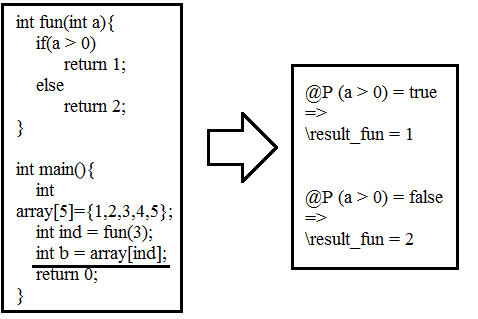
\includegraphics[keepaspectratio, width=8cm, height=7cm]{ex1}
\end{figure}
